\scanpage{219}
$X$ \deleted{schéma} préschéma de type fini \inserted{normal} irréductible sur corps $k$

$\unsure{v|\nu},\unsure{w|\omega}$ deux places archimédiennes de \deleted{\unsure{le}} $X$, d'où foncteurs fibres
$\xi_{\unsure{v|\nu}}^{\mathbf Z},\xi_{\unsure{w|\omega}}^{\mathbf Z}$.
Question: a) \inserted{Quand} sont-ils isomorphes?
b) \deleted{Est-il vrai que} Quand est-il vrai que pour tte sous-catégorie \inserted{mult.} de t.f. de $\mathcal M(X)$, les restrictions de ces foncteurs à $\mathcal M_\alpha(X)$ sont isomorphes?

Nous pouvons supposer, quitte à remplacer $k$ par
\deleted{\unsure{Soient $v',w'$ les}}
sa clôture alg. dans $k(X)$, que $k$ est alg. clos dans $k(X)$ [\unsure{utilise|utiliser} le fait $X$ \uline{normal}!]
donc $X$ est géom\textsuperscript{t} \unsure{irrid.|irred.} sur $k$.
Soit \deleted{$k_0$} \inserted{$k_0$ la clôture alg. de $\mathbf Q$ dans $k$.}
\deleted{le corps des \unsure{coïncidences} des places (= val. abs.) induites sur $k$, \unsure{envisagées}}
\inserted{\uline{contient la clôture alg. $\unsure{E}$ de $\mathbf Q$ dans $k$} (p.ex. $k_0$ alg. fermé dans $k$).}
\deleted{1) $k_0$ est algébriquement fermé dans $k$. Alors}
\inserted{1°) $\unsure{v|\nu},\unsure{w|\omega}$ coïncident sur $k_0$.}

\[
\text{a)}\quad \xi_{\unsure{v|\nu}}^{\mathbf Z}|\mathcal M_\alpha(X)
\simeq \xi_{\unsure{w|\omega}}^{\mathbf Z}|\mathcal M_\alpha(X)
\quad\text{pour }\forall\ \alpha.
\]

\margin{\diagram{\begin{tikzcd}[column sep=13pt,row sep=12pt]
&X_0\arrow[r,no head]\arrow[d,no head]&X\arrow[d,no head]\\
k_0\arrow[r,no head]&A_0\arrow[r,no head]&k
\end{tikzcd}}}

En effet, $X$ et $\mathcal M_\alpha(X)$ proviennent de $X_0$, \inserted{$\mathcal M_\alpha(X_0)$}, de type fini sur $A_0$, \inserted{$k_0$}$k$-alg. de type fini de $k$,
\deleted{$X_0\longrightarrow\operatorname{Spec}A_0$ fid plt \unsure{et irred sur} $A_0$}\inserted{\unsure{conn et}} $^*$
\deleted{\unsure{et}}
On est ramené au cas où $k=\unsure{k_0|E_0}$, où on obtient le résultat voulu grâce au groupe fondamental transcendant.

\margin{\deleted{\diagram{\begin{tikzcd}[column sep=12pt,row sep=10pt]
&\unsure{X_0}\arrow[r,no head]\arrow[d,no head]&X\arrow[d,no head]\\
E\arrow[r,no head]\arrow[dr]&\unsure{k_0}\arrow[r,no head]\arrow[d,no head]&k\\
& A_0\arrow[r,no head]&\unsure{E|\mathbf Z}\\
&\unsure{\mathbf Q}\arrow[u,no head]\arrow[ur,no head]&
\end{tikzcd}}}}

\deleted{\unsure{Alors}}
b) Si \deleted{$k=k_0$}\inserted{$\unsure{v|\nu}$ et $\unsure{w|\omega}$ coïncident sur $k$,}
cet argument montre que
$\xi_{\unsure{v|\nu}}^{\mathbf Z}\simeq\xi_{\unsure{w|\omega}}^{\mathbf Z}$.
\inserted{sinon, mais \unsure{si on suppose} $k$ est \illegible{1}}
\deleted{Si $k\ne k_0$, \unsure{on peut} $\xi_{\unsure{v|\nu}}^{\mathbf Z}\ne\xi_{\unsure{w|\omega}}^{\mathbf Z}$, \unsure{géom} \illegible{1}}

\margin{$^*$ on peut supposer $X_0\to\operatorname{Spec}A_0$ fid plt \unsure{géomt connexe}, et
\diagram{\begin{tikzcd}[column sep=8pt]\operatorname{Spec}(A_0)\arrow[r,no head]&k_0\end{tikzcd}}
géom connexe, donc
\diagram{\begin{tikzcd}[column sep=8pt]X_0\arrow[r,no head]&\operatorname{Spec}k_0\end{tikzcd}}
géom connexe.}
\figure{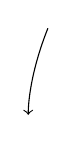
\begin{tikzpicture}\draw[->] (0,1.1) .. controls (-.2,.6) and (-.25,.2) .. (-.25,0);\end{tikzpicture}}

\margin{218}
